\documentclass{beamer}
\usepackage{fontspec}
\usepackage{bibentry}
\usepackage{graphicx}

\setmainfont{Sarasa-Fixed-Slab-SC-Regular}
\setsansfont{HelveticaNeue}
\setbeamertemplate{frametitle}[default][center]

\mode<presentation> {

% The Beamer class comes with a number of default slide themes
% which change the colors and layouts of slides. Below this is a list
% of all the themes, uncomment each in turn to see what they look like.

\usetheme{default}
%\usetheme{AnnArbor}
%\usetheme{Antibes}
%\usetheme{Bergen}
%\usetheme{Berkeley}
%\usetheme{Berlin}
%\usetheme{Boadilla}
%\usetheme{CambridgeUS}
%\usetheme{Copenhagen}
%\usetheme{Darmstadt}
%\usetheme{Dresden}
%\usetheme{Frankfurt}
%\usetheme{Goettingen}
%\usetheme{Hannover}
%\usetheme{Ilmenau}
%\usetheme{JuanLesPins}
%\usetheme{Luebeck}
%\usetheme{Madrid}
%\usetheme{Malmoe}
%\usetheme{Marburg}
%\usetheme{Montpellier}
%\usetheme{PaloAlto}
%\usetheme{Pittsburgh}
%\usetheme{Rochester}
%\usetheme{Singapore}
%\usetheme{Szeged}
%\usetheme{Warsaw}

% As well as themes, the Beamer class has a number of color themes
% for any slide theme. Uncomment each of these in turn to see how it
% changes the colors of your current slide theme.

%\usecolortheme{albatross}
%\usecolortheme{beaver}
%\usecolortheme{beetle}
%\usecolortheme{crane}
%\usecolortheme{dolphin}
\usecolortheme{dove}
%\usecolortheme{fly}
%\usecolortheme{lily}
%\usecolortheme{orchid}
 %\usecolortheme{rose}
%\usecolortheme{seagull}
%\usecolortheme{seahorse}
%\usecolortheme{whale}
%\usecolortheme{wolverine}

%\setbeamertemplate{footline} % To remove the footer line in all slides uncomment this line
%\setbeamertemplate{footline}[page number] % To replace the footer line in all slides with a simple slide count uncomment this line

%\setbeamertemplate{navigation symbols}{} % To remove the navigation symbols from the bottom of all slides uncomment this line
}

\usepackage{graphicx} % Allows including images
\usepackage{booktabs} % Allows the use of \toprule, \midrule and \bottomrule in tables

%----------------------------------------------------------------------------------------
%	TITLE PAGE
%----------------------------------------------------------------------------------------

\title[Short title]{Exercise recommender system based on knowledge graph and knowledge modeling} % The short title appears at the bottom of every slide, the full title is only on the title page

\author{ Wangzhihui Mei 2019124044} % Your name
\institute[JI] % Your institution as it will appear on the bottom of every slide, may be shorthand to save space
{
CCNU-UOW JI \\ % Your institution for the title page
\medskip
\textit{maywzh@gmail.com} % Your email address
}
\date{\today} % Date, can be changed to a custom date

\begin{document}

\begin{frame}
\titlepage % Print the title page as the first slide
\end{frame}

\begin{frame}
\frametitle{Overview} % Table of contents slide, comment this block out to remove it
\tableofcontents % Throughout your presentation, if you choose to use \section{} and \subsection{} commands, these will automatically be printed on this slide as an overview of your presentation
\end{frame}

%----------------------------------------------------------------------------------------
%	PRESENTATION SLIDES
%----------------------------------------------------------------------------------------

%------------------------------------------------
\section{Introduction}
\subsection{Background}
\begin{frame}
  \frametitle{Background}
  The educational method of teaching students in accordance with their aptitude has a history of more than 2,000 years in our country, but in the context of our country’s exam-oriented education, it is really easy to say that it is difficult to formulate a personalized learning plan based on students' different cognitive levels learning abilities and their own qualities. When traditional thinking is combined with cutting-edge technology, the feasibility of teaching students in accordance with their aptitude has been greatly improved. After the intervention of AI, there are two ways to achieve personalized learning.

\end{frame}

\subsection{Basic Methodology}
\begin{frame}
  \frametitle{Basic Methodology}
  \begin{itemize}
    \item Analyze content and build a knowledge graph.
    \item Adaptive learning to realize intelligent recommendation.
  \end{itemize}
\end{frame}

%------------------------------------------------



%------------------------------------------------

\section{Knowledge graph}
% \subsection{Introduction}
% \begin{frame}
%   \frametitle{Analysis}
%   \begin{itemize}
%     \item Privacy should be kept on local device except for being infected
%     \item All data transmission process should be encrypted
%     \item The client is anonymous to other clients and servers
%   \end{itemize}

% \end{frame}
% \subsection{Proposed Protocol}
\begin{frame}%[allowframebreaks] 
  \frametitle{Knowledge graph\cite{1}}
  \begin{figure}
    \centering
    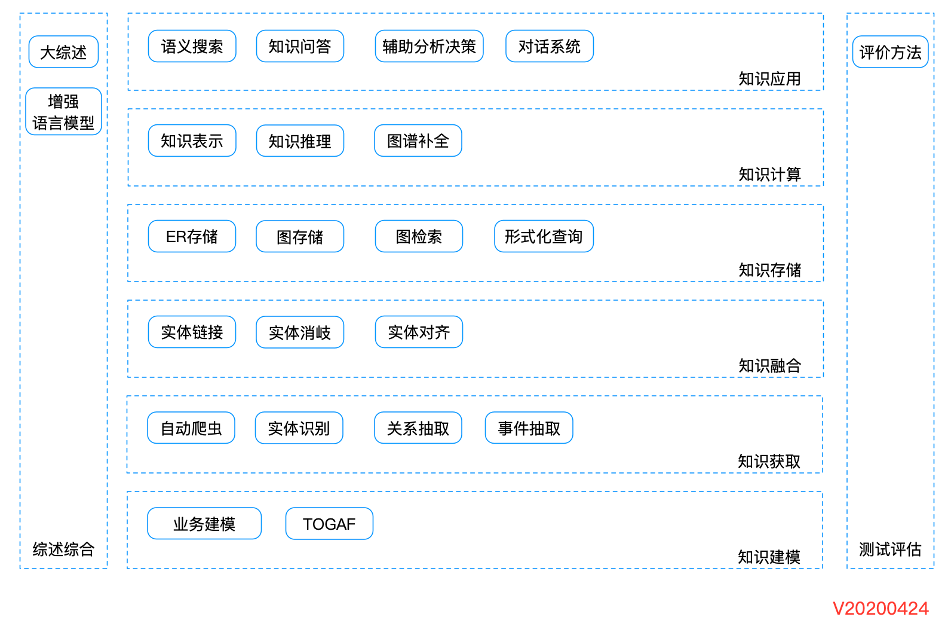
\includegraphics[height=0.6\textwidth]{figure/kg0}
    \caption{KG research fields}
  \end{figure}
  
  % \begin{figure}[]
  %   \centering
  %   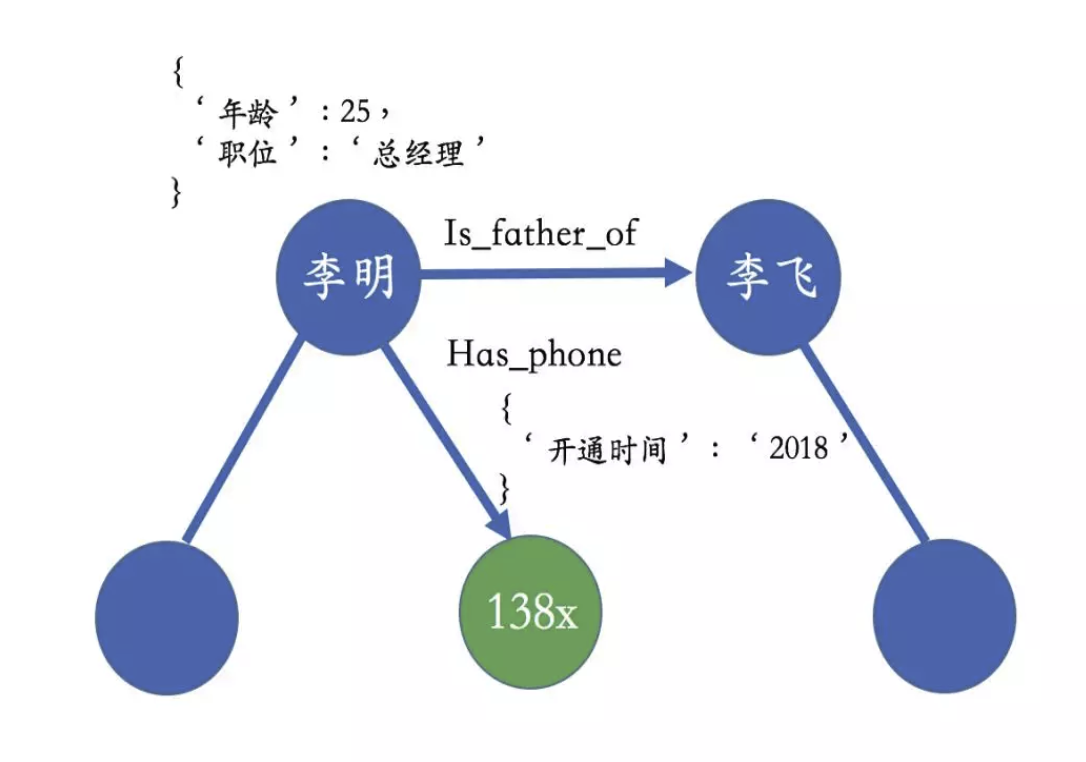
\includegraphics[height=0.7\textheight]{figure/kg11}
  %   \caption{Tri-tuple}
  % \end{figure}

\end{frame}

% \begin{frame}
%   \frametitle{Literature review}
%   \begin{itemize}
%     \item Knowledge Representation, Acquisition and Applications\cite{1}
%   \end{itemize}

% \end{frame}


\subsection{Literature review}
\begin{frame}
  \frametitle{KG Completion}
  Alberto et. all utilized recurrent neural networks to learn time-aware representations of relation types which
  can be used in conjunction with existing latent factorization methods.\cite{1}

  Yao et. all introduced the work of knowledge base completion. Combined with the pre-training model BERT, it can integrate richer context representation into the model, and achieve SOTA effects in tasks such as triple classification, link prediction, and relationship prediction.\cite{2}
\end{frame}

\begin{frame}
  \frametitle{Cognitive Diagnosis}
  Wang et. all proposed neural cognitive diagnosis method for intelligent education system. \cite{3}
\end{frame}

\begin{frame}
  \frametitle{Knowledge Tracing}
  \begin{itemize}
    \item Individualized Bayesian Knowledge Tracing Models\cite{4}
    \item Deep Knowledge Tracing\cite{5}
    \item Tracking Knowledge Proficiency of Students with Educational Priors\cite{6}
  \end{itemize} 
  \cite{3}
\end{frame}

\begin{frame}[allowframebreaks]
  \frametitle{References}
  \footnotesize{
  \begin{thebibliography}{99} % Beamer does not support BibTeX so references must be inserted manually as below
      \bibitem{1}
      Ji, S., Pan, S., Cambria, E., Marttinen, P., \& Yu, P. S.  (2020). 
      \newblock A survey on knowledge graphs: Representation, acquisition and applications.
      \newblock arXiv preprint arXiv:2002.00388.
      \bibitem{2}
      Liang Yao and Chengsheng Mao and Yuan Luo.  (2019). 
      \newblock KG-BERT: BERT for Knowledge Graph Completion.
      \newblock arXiv preprint arXiv:1909.03193.
      \bibitem{3}
      Wang F, Liu Q, Chen E, et al. 
      \newblock Neural Cognitive Diagnosis for Intelligent Education Systems[J]. 
      \newblock arXiv preprint arXiv:1908.08733, 2019.
      \bibitem{4}
      Yudelson M V, Koedinger K R, Gordon G J. 
      \newblock Individualized bayesian knowledge tracing models[C]
      \newblock International conference on artificial intelligence in education. Springer, Berlin, Heidelberg, 2013: 171-180.  
      \bibitem{5}
      Piech C, Bassen J, Huang J, et al.
      \newblock Deep knowledge tracing.
      \newblock In Advances in neural information processing systems (pp. 505-513).
      \bibitem{6}
      Chen Y, Liu Q, Huang Z, et al. 
      \newblock Tracking knowledge proficiency of students with educational priors[C]
      \newblock Proceedings of the 2017 ACM on Conference on Information and Knowledge Management. 2017: 989-998.
    \end{thebibliography}

  }
  \end{frame}

\begin{frame}
\Huge{\centerline{The End}}
\end{frame}

%----------------------------------------------------------------------------------------

\end{document} 